%----------------------------------------------------------------------------------------
%	PACKAGES AND OTHER DOCUMENT CONFIGURATIONS
%------------------------------------------------------------------------
\documentclass[11pt]{article}
\usepackage[utf8]{inputenc} % Required for inputting international characters
\usepackage[T1]{fontenc} % Output font encoding for international characters
\usepackage{mathpazo} % Palatino font
\usepackage[czech]{babel} % Czech
\usepackage{graphicx}  % Graphics
\usepackage{amsmath}
\usepackage{pdfpages}

\begin{document}
	
	%----------------------------------------------------------------------------------------
	%	TITLE PAGE
	%----------------------------------------------------------------------------------------
	
	\begin{titlepage} % Suppresses displaying the page number on the title page and the subsequent page counts as page 1
		\newcommand{\HRule}{\rule{\linewidth}{0.5mm}} % Defines a new command for horizontal lines, change thickness here
		
		\center % Centre everything on the page
		
		%------------------------------------------------
		%	Headings
		%------------------------------------------------
		
		\textsc{\LARGE České vysoké učení technické v Praze}\\[1.5cm] % Main heading such as the name of your university/college
		
		\textsc{\Large Algoritmy digitální kartografie a GIS}\\[0.5cm] % Major heading such as course name
		
		\textsc{\large Katedra geomatiky}\\[0.5cm] % Minor heading such as course title
		
		%------------------------------------------------
		%	Title
		%------------------------------------------------
		
		\HRule\\[0.4cm]
		
		{\huge\bfseries Úloha č. 2: Konvexní obálky}\\[0.4cm] % Title of your document
		
		\HRule\\[1.5cm]
		
		%------------------------------------------------
		%	Author(s)
		%------------------------------------------------
		
		
		
		
		% If you don't want a supervisor, uncomment the two lines below and comment the code above
		Monika \textsc{Křížová} % Your name
		
		Marek \textsc{Hoffmann}
		
		%------------------------------------------------
		%	Date
		%------------------------------------------------
		
		\vfill\vfill\vfill % Position the date 3/4 down the remaining page
		
		{\large 06.11.2021} % Date, change the \today to a set date if you want to be precise
		
		%------------------------------------------------
		%	Logo
		%------------------------------------------------
		
		%\vfill\vfill
		%\includegraphics[width=0.2\textwidth]{placeholder.jpg}\\[1cm] % Include a department/university logo - this will require the graphicx package
		
		%----------------------------------------------------------------------------------------
		
		\vfill % Push the date up 1/4 of the remaining page
		
	\end{titlepage}
	
	%----------------------------------------------------------------------------------------
	
	
	%----------------------------------------------------------------------------------------
	%	TABLE OF CONTENT
	%----------------------------------------------------------------------------------------
	
	\tableofcontents
	%\thispagestyle{empty}
	
	\clearpage
	
	%----------------------------------------------------------------------------------------
	%	ZADÁNÍ
	%----------------------------------------------------------------------------------------
	
	\section{Zadání}
	Vytvořte aplikaci s grafickým uživatelským rozhraním, která bude ze souboru načítat polygony budov a následně je bude generalizovat na obdélníky s plochou odpovídající generalizované budově a bude vytvářet konvexní obálky. Hlavní směry budov budou určeny metodami Minimum Area Enclosing Rectangle a Wall Average.
	
	Přesné zadání je vloženo na následující stranu.
	
	
	
	
	%---------------------------------------------------------------------
	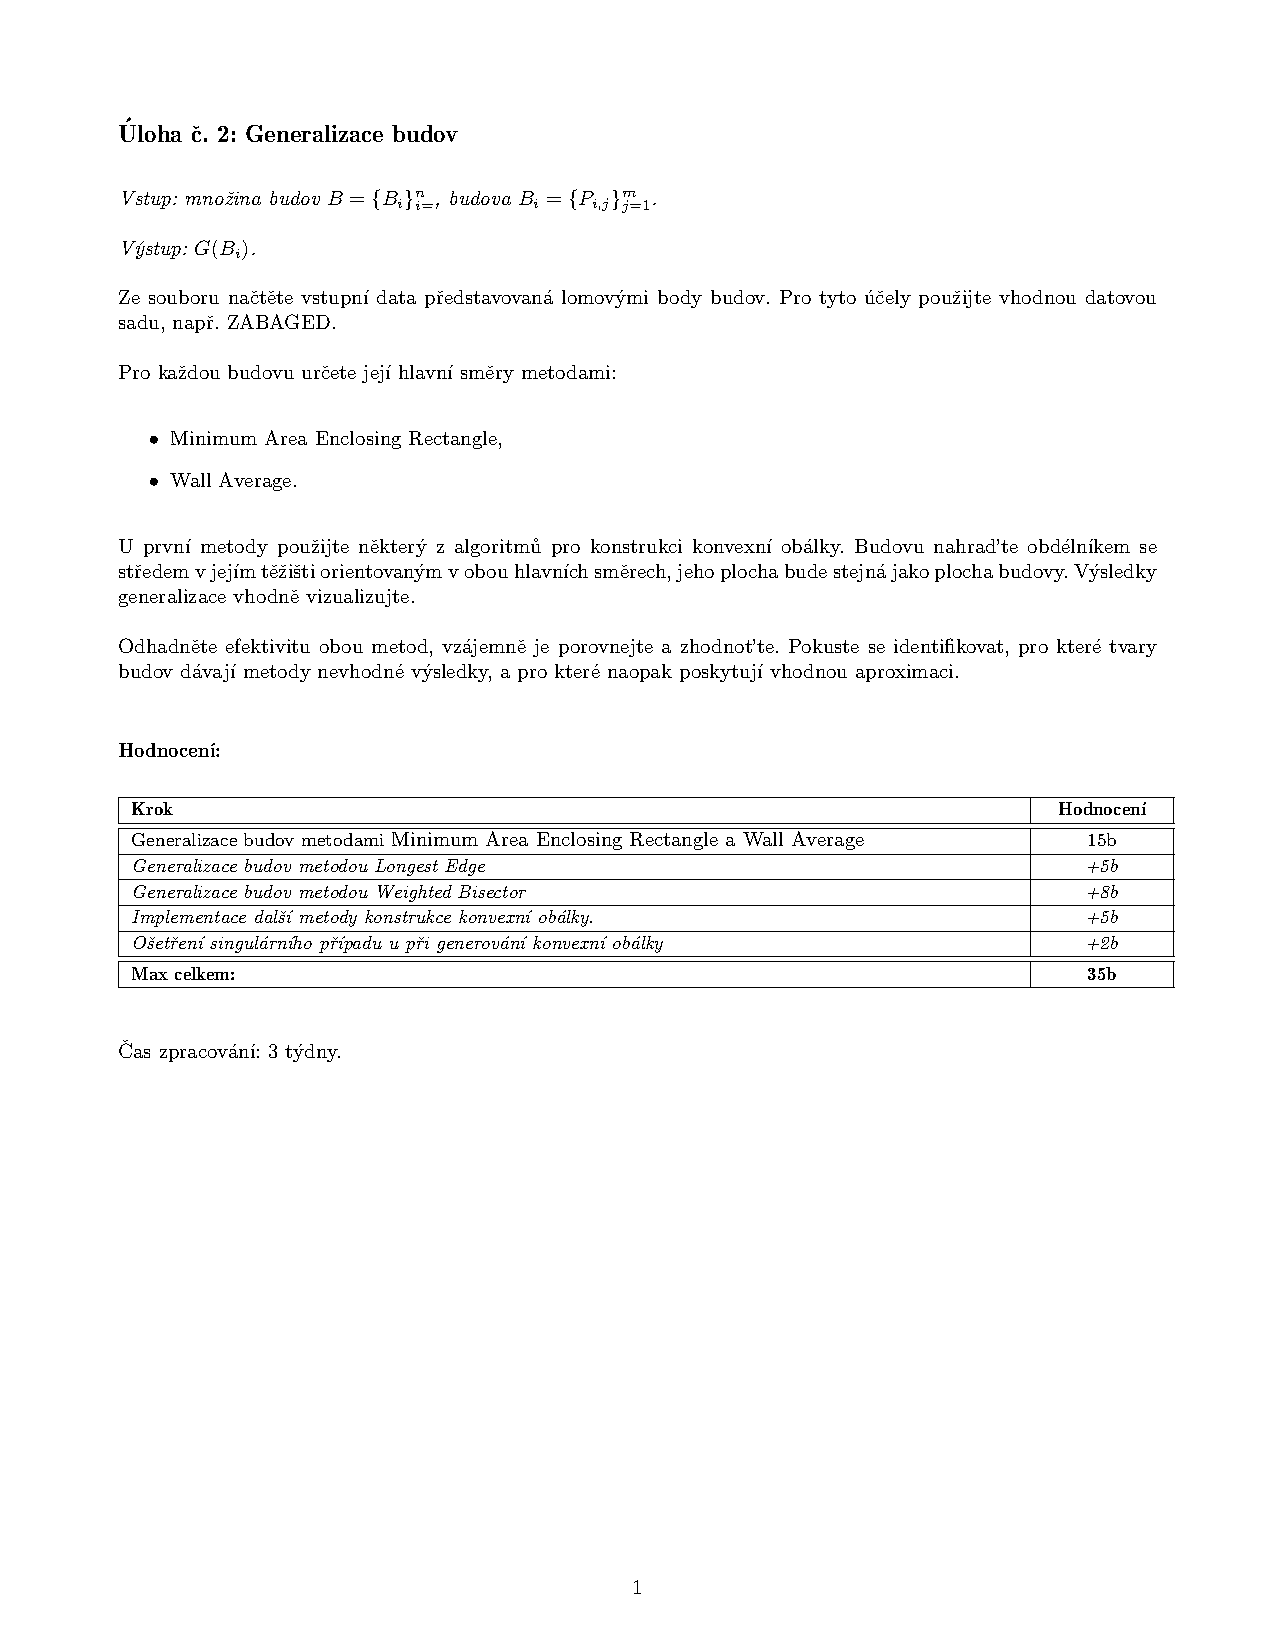
\includepdf{adkcv2.pdf}
	
	
	
	%---------------------------------------------------------------------
	
	%----------------------------------------------------------------------------------------
	%	ÚDAJE O BONUSOVÝCH ÚLOHÁCH
	%----------------------------------------------------------------------------------------
	
	\section{Údaje o bonusových úlohách}
	Zpracovány byly celkem 3 bonusové úlohy ze 4 zadaných.
	
	\begin{itemize}
		\item Generalizace budov metodou Longest Edge +5b
		\item Generalizace budov metodou Weighted Bisector +8b
		\item Implementace další metody konstrukce konvexní obálky. +5b
	\end{itemize}
	
	Generalizace budov metodou Longest Edge byla implementována ve třídě Algorithms, je možné ji spustit pomocí tlačítka Building simplify po předchozím výběru v comboBoxu umožňujícího výběr metody generalizace polygonu.
	
	Generalizace budov metodou Weighted Bisector byla stejně jako metoda Longest Edge implementována ve třídě Algorithms a taktéž je ji možné spustit pomocí tlačítka Building simplify po předchozím výběru v comboBoxu umožňujícího výběr metody generalizace polygonu.
	
	Pro implementaci další metody konstrukce konvexní obálky byla vybrána metoda Quick Hull, jež byla přidána do třídy Algorithms. Pro její spuštění je nutné vybrat tuto metodu v náležitém comboBoxu a následně stisknout tlačítko Create convex hull.
	
	
	%----------------------------------------------------------------------------------------
	%	POPIS PROBLÉMU
	%----------------------------------------------------------------------------------------
	
	\section{Popis problému}
	Generalizace je v kartografii velmi důležitý proces, který je používán například při změně měřítka mapy, změně jejího účelu nebo pro zlepšení grafické přehlednosti. Generalizace může být provedena několika různými metodami, v řešené úloze byla aplikována tzv. geometrická generalizace, jež spočívá ve zjednodušení tvaru objektu. Objekty (v této úloze budovy) byly generalizovány na obdélníky s plochou odpovídající ploše původních objektů.
	
	Jednotlivé generalizační algoritmy hledají hlavní směr natočení budovy, po nalezení tohoto směru se vytvoří opsaný obdélník s minimálním obsahem, jež je natočený do tohoto směru (dále pod zkratkou MMB). MMB se následně zmenší tak, aby byla jeho plocha totožná s plochou generalizovaného objektu. 
	
	%----------------------------------------------------------------------------------------
	%	POPIS ALGORITMŮ
	%----------------------------------------------------------------------------------------
	
	\section{Popisy algoritmů}
	\subsection{Tvorba konvexní obálky}
	\subsubsection{Jarvis scan}
	
	Prvním krokem při tvorbě konvexní obálky $\mathcal{H}$ metodou Jarvis scan je nalezení pivotu \textit{q}. Tento bod je bod s nejmenší souřadnicí \textit{y} v množině bodů \textit{S}. Dalším krokem je nalezení bodu \textit{p}, jež svírá největší úhel s rovnoběžkou s osou \textit{x} procházející bodem \textit{q}. Nalezený bod se přidá do $\mathcal{H}$ a opět se hledá bod, jež bude svírat s předchozím bodem největší úhel. Tímto způsobem se do $\mathcal{H}$ přidávají body do okamžiku, kdy by byl přidávaným bodem bod \textit{q}. Tato metoda je velmi jednouchá, ale kvůli časové náročnosti nevhodná pro velké množiny bodů.
	
	\subsubsection{Quick Hull}
	
	V algoritmu Quick Hull je nejprve nutné seřadit množinu bodů \textit{S} podle souřadnice \textit{x} a následně ze setříděného souboru vybrat dva body, tzv. pivoty. Bod \textit{$ q_{1} $} je bodem s nejmenší souřadnicí \textit{x}, bod \textit{$ q_3 $} má naopak souřadnici x ze souboru bodů \textit{S} největší. Konvexní obálka $\mathcal{H}$ se vytváří ze dvou částí – horní ($\mathcal{H_U}$) a spodní $\mathcal{H_L}$ konvexní obálky. 
	Do $\mathcal{H_U}$ se přidávají body ležící nalevo od spojnice pivotů \textit{$ q_{1} $} a \textit{$ q_{3} $}, do $\mathcal{H_L}$ naopak body ležící na pravé straně od spojnice týchž bodů.
	
	Posledním krokem je spojení obou částí konvexní obálky do výsledné množiny $\mathcal{H}$. Nejprve se do $\mathcal{H}$ přidá bod \textit{$ q_3 $}, poté se provede rekurze $\mathcal{H_U}$, pomocí níž se do $\mathcal{H}$ přidají body z horní části konvexní obálky, poté se přidá bod \textit{$ q_{1} $} a posledním krokem je provedení rekurze $\mathcal{H_L}$, díky níž se do konvexní obálky přidají i body ze spodní části konvexní obálky.
	
	
	\subsection{Generalizace budov}
	\subsubsection{Minimum Enlosing Rectangle}
	Algoritmus se snaží vyhledat takovou hranu konvexní obálky $\mathcal{H}$, aby po vytvoření opsaného obdélníka s jednou stranou kolineární s touto hranou měl takto vytvořený obdélník minimální plochu.
	
	Algoritmus využívá již zkonstruovanou konvexní obálku $\mathcal{H}$, pro jejíž hrany jsou vypočítávány směrnice $\sigma$ hrany \textit{e}: 
	
	\begin{equation}
		\tan\sigma=\frac{d_x}{d_y}, 
	\end{equation}
	kde $d_{x}$ a $d_{y}$ jsou souřadnicové rozdíly počátečního a koncového bodu hrany konvexní obálky $\mathcal{H}$. Všechny body množiny \textit{S} se následně pomocí matice rotace \textit{R} otočí o úhel $-\sigma$:
	
	\begin{equation}
		S_R=R(-\sigma)S 
	\end{equation}
	
		Pro otočené body množiny se vytvoří MMB s následujícími souřadnicemi vrcholů:
		
		\begin{equation}
			V_1 = [\underline{x}, \underline{y}], V_2 = [\overline{x}, \underline{y}],
			V_3 = [\overline{x}, \overline{y}],
			V_4 = [\underline{x}, \overline{y}],
		\end{equation}
		
		kde $\underline{x},\overline{x},\underline{y}, \overline{x}$ jsou minimální a maximální souřadnice natočených bodů množiny \textit{$ S_R $}. Vypočte se plocha vytvořeného \textit{MMB}:
		
		\begin{equation}
			A = (\overline{x}-\underline{x})(\overline{y}-\underline{y}),
		\end{equation}
		
		jež se následně porovná s minimální uloženou plochou. Je-li vypočtená plocha \textit{A} menší než je plocha minimální, uloží se jako nové minimum. Dále se uloží pro tuto plochu uloží úhel $ \sigma_{min} $ a \textit{$MMB_{min}$}. Po ukončení výpočtu 
		totoho cyklu je již vypočten výsledný úhel natočení budovy $ \sigma_{min} $. Následně je nutné \textit{MMB} natočit o tento úhel a zmenšit tak, aby byla plocha \textit{MMB} rovna ploše generalizovaného polygonu. Tento postup bude používán i pro další metody.
		
		\textit{$MMB_{min}$} se otočí o úhel $ \sigma_{min} $:  
		
		\begin{equation}
		\mathcal{R} = R(\sigma_{min})MMB_{min}, 
		\end{equation}
		
		následně se jeho plocha proporcionálně zmenší vůči těžišti tak, aby byla rovna ploše generalizovaného polygonu. Nejprve je nutné vypočítat poměr \textit{k} plochy \textit{$A_b$} generalizované budovy a plochy \textit{A} \textit{MMB}
		
		\begin{equation}
			k = \dfrac{A_b}{A}.
		\end{equation}
		
		Souřadnice těžiště \textit{T} jsou aritmetickým průměrem souřadnic vrcholů $\mathcal{R}$. Vypočítají se nové vrcholy \textit{V} obdélníku $\mathcal{R}_r$:
		
		\begin{equation}
			V_i = T + \sqrt{k}u_i, 
		\end{equation}
	
		kde \textit{$u_i$} jsou směrové vektory vrcholů a těžiště odvozené z Pythagorovy věty:
		
		\begin{equation}
			u_i = V_i - T 
		\end{equation}
	
	

		\subsubsection{Metoda Wall Average}
		Metoda je velmi komplexní a citlivá na nepravé úhly. Pro každou hranu je pro výsledky operace mod() vypočítáván vážený průměr, v němž je vahou délka hrany.
		
		Pro každou hranu budovy se zredukuje směrnice $\sigma$:
		
		\begin{equation}
			\Delta\sigma = \sigma_i - \sigma',
		\end{equation} 
		kde $ \sigma_i $ je směrnice hrany vypočtená dle vztahu (1) a $ \sigma' $ je směrnice první hrany vypočtená dle vztahu (1). 
		
		V dalším kroku se vypočítá zaokrouhlený podíl:
		\begin{equation}
			k_i = \bigg[\frac{2\Delta\sigma_i}{\pi}\bigg]
		\end{equation}
		
		a následně se dopočítá zbytek po dělení:
		
		\begin{equation}
			r_i = \Delta\sigma_i - k_i\dfrac{\pi}{2}.
		\end{equation}
		
		Výsledný směr natočení budovy roven:
		\begin{equation}
			\sigma=\sigma'+\sum\frac{r_is_i}{s_i}.
		\end{equation}
	
		Následně se vytvoří MMB, který se otočí o úhel $ \sigma $ a zmenší do požadované plochy. Tento postup byl již shrnut v kapitole 4.2.1.
		
		\subsubsection{Metoda Longest Edge}
		Hlavní směrem budovy se dle této metody rozumí směrnice nejdelší hrany budovy, druhý směr je kolmý na směr hlavní. 	
		Pomocí cyklu se postupně vypočítává délka \textit{d} všech hran generalizované budovy, postupně se zjišťuje, je-li vypočtená délka větší než je dosavadně největší uložená délka.
		
		\begin{equation}
			d = \sqrt{d_x ^2 + d_y ^2}
		\end{equation}
		
		Následně se vytvoří MMB, který se otočí o úhel $ \sigma $ a zmenší do požadované plochy. Tento postup byl již shrnut v kapitole 4.2.1.
		
		\subsubsection{Metoda Weighted Bisector}				 
		Algoritmus hledá dvě nejdelší úhlopříčky generalizované budovy, pro tyto dvě úhlopříčky se následně vypočítají směrnice (rovnice (1)) a délky hran (rovnice (13)). Výsledný směr se získá z váženého průměru:
		
		\begin{equation}
			\sigma = \frac{s_1\sigma_1+s_2\sigma_2}{s_1+s_2}.
		\end{equation}
	
		Následně se vytvoří MMB, který se otočí o úhel $ \sigma $ a zmenší do požadované plochy. Tento postup byl již shrnut v kapitole 4.2.1.
		
			
		%----------------------------------------------------------------------------------------
		%	PROBLEMATICKÉ SITUACE
		%----------------------------------------------------------------------------------------
		
		\section{Problematické situace}
		Během práce na úloze se vyskytly problémy při načítání dat, které byly uloženy v souřadních S-JTSK, z něhož je bylo nutné transformovat do souřadnic plátna pro vykreslování. 
		
		Prvním krokem byla změna měřítka souřadnic a zaměnění souřadnice \textit{x} za \textit{y} a naopak, následovalo získání minimálních a maximálních souřadnic \textit{x} a \textit{y} bodů množiny \textit{S}. Z vypočtených minim a maxim se následně vypočítal rozsah mezi těmito souřadnicemi, kterým se vydělil rozsah plátna, čímž se získalo měřítko, jímž se následně souřadnice vynásobily.
		
		
		%----------------------------------------------------------------------------------------
		%	VSTUPNÍ DATA
		%----------------------------------------------------------------------------------------
		
		
		\section{Vstupní data}
		Polygonová mapa se do projektu nahrává z textového souboru, ve kterém jsou uloženy souřadnice lomových bodů budov v souřadnicovém systému S-JTSK s centimetrovou přesností. Data byla získána ze systému ZABAGED, pomocí QGISu se vyexportovaly souřadnice do csv souboru, jehož formát se pak pomocí jednoduchých funkcí v MS Excel upravil do špagetového modelu. Pro úspěšné načtení souboru musí data splňovat specifický formát, bez něhož nebude zajištěno správné načítání dat.  
		
		Vrcholy polygonů jsou načítány postupně řádek po řádku, přičemž musí v nahrávaném souboru platit následující pravidla:    
		
		\begin{itemize}
			\item každý vrchol polygonu je definován na jednotlivém řádku,
			\item na řádku je pořadí proměnných id >> y >> x   ,  hodnoty jsou od sebe odděleny  jednou mezerou,
			\item id je identifikátor jednotlivých vrcholů polygonu, x a y jsou souřadnice vrcholů polygonu,    
			\item nový polygon má vždy hodnotu id prvního vrcholu rovnu 1, od této hodnoty  se  postupně načítají body, a  to až do okamžiku,  kdy program dojde  k dalšímu identifikátoru s označením 1.   
		\end{itemize}
		
		\begin{figure}[htbh]
			\centering
			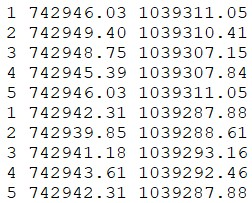
\includegraphics[scale=1]{images/vstup_data_U2.jpg} 
			\caption{Špagetový model vstupního souboru}
			\label{fig:vstup.}
		\end{figure} 
		
		Souřadnice byly následně transformovány z S-JTSK do souřadnicového systému widgetu a změněno bylo měřitko tak, aby se zobrazovala oblast se  zobrazovanými polygony s maximálním přiblížením. Tento postup byl již popsán v kapitole 4.
		
		\clearpage

		
		%----------------------------------------------------------------------------------------
		%	VÝSTUPNÍ DATA
		%----------------------------------------------------------------------------------------
		
		\section{Výstupní data}
		
		Po načtení souboru lze nad polygony provádět dva druhy operací. Po stisknutí tlačítka \textit{Create convex hull} se vytvoří konvexní obálky nad jednotlivými polygony. V combo boxu lze vybrat, zdali se konvexní obálka vytvoří metodou \textit{Jarvis scan} nebo \textit{Quick hull}. Výsledek obou metod je stejný a zobrazuje ho následující obrázek \ref{fig:app_convexHull}.
		
		\begin{figure}[htbh]
			\centering
			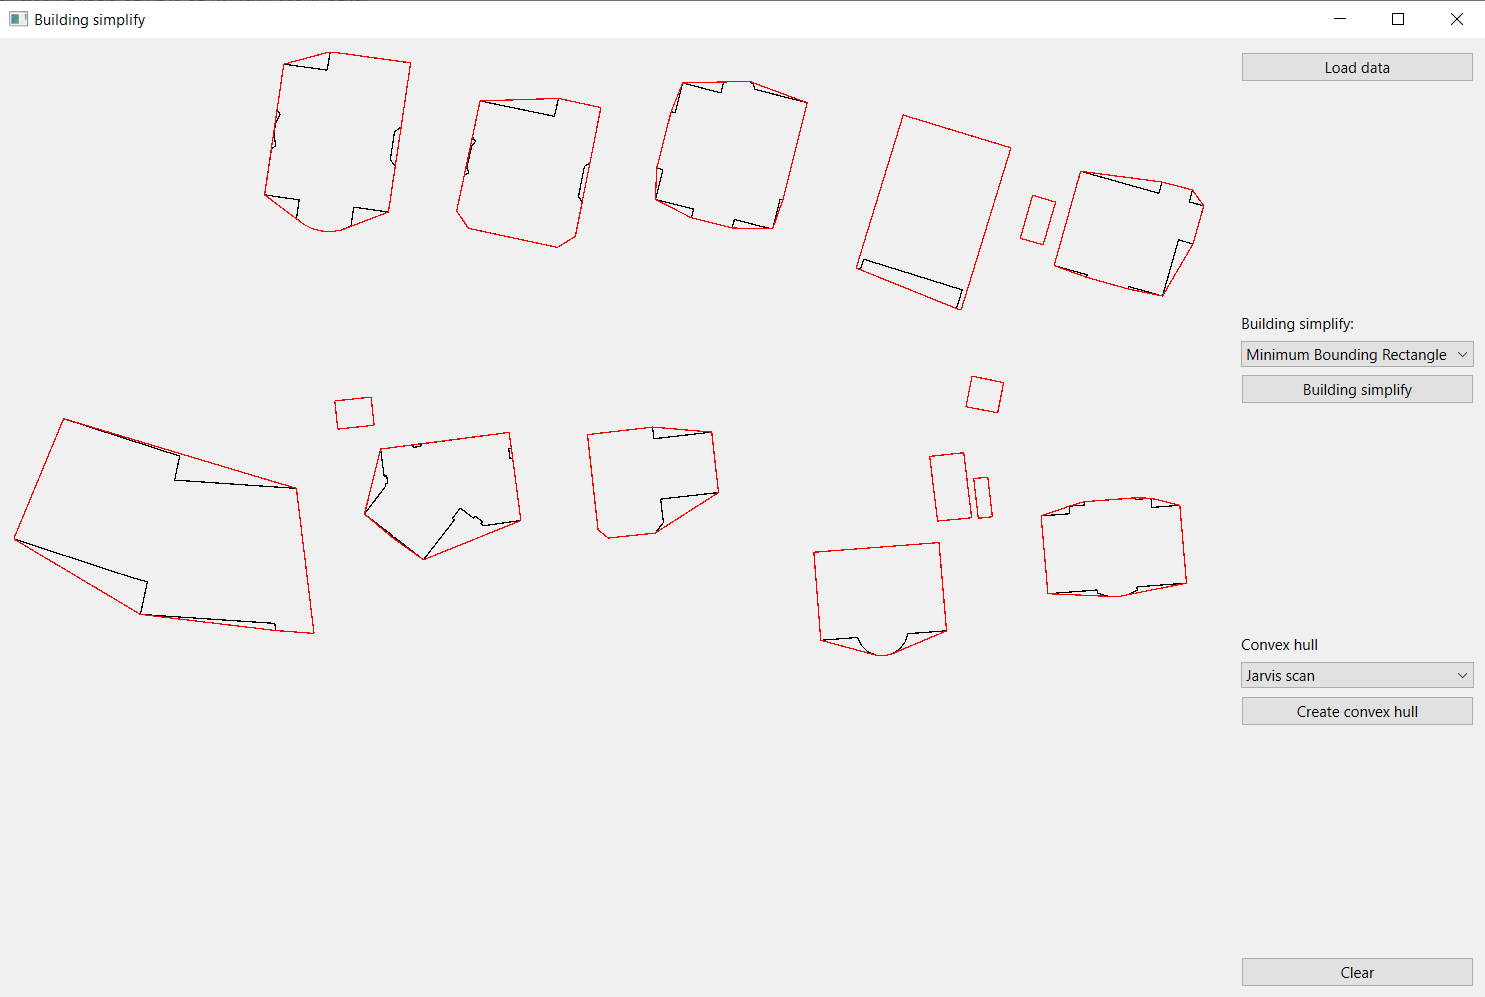
\includegraphics[scale=0.4]{images/U2_aplikace_ConvexHull.png} 
			\caption{Konvexní obálka nad polygony}
			\label{fig:app_convexHull}
		\end{figure} 
		
		Druhým typem operací, které lze v aplikaci provádět, je generalizace budov. Po stisknutí tlačítka \textit{Building simplify} je možné provést čtyři následující metody pro výpočet hlavního směru orientace generalizované budovy.
		
		\begin{itemize}
			\item Minimum Area Enclosing Rectangle 
			\item Wall Avarage 
			\item Longest Edge
			\item Weighted Bisector 
		\end{itemize}
		
		Výsledky jednotlivých metod zobrazují obrázky \ref{fig:app_MAER}, \ref{fig:app_WallAvarage}, \ref{fig:app_LongestEdge}, \ref{fig:app_WeightedBisector}.
		\begin{figure}[htbh]
			\centering
			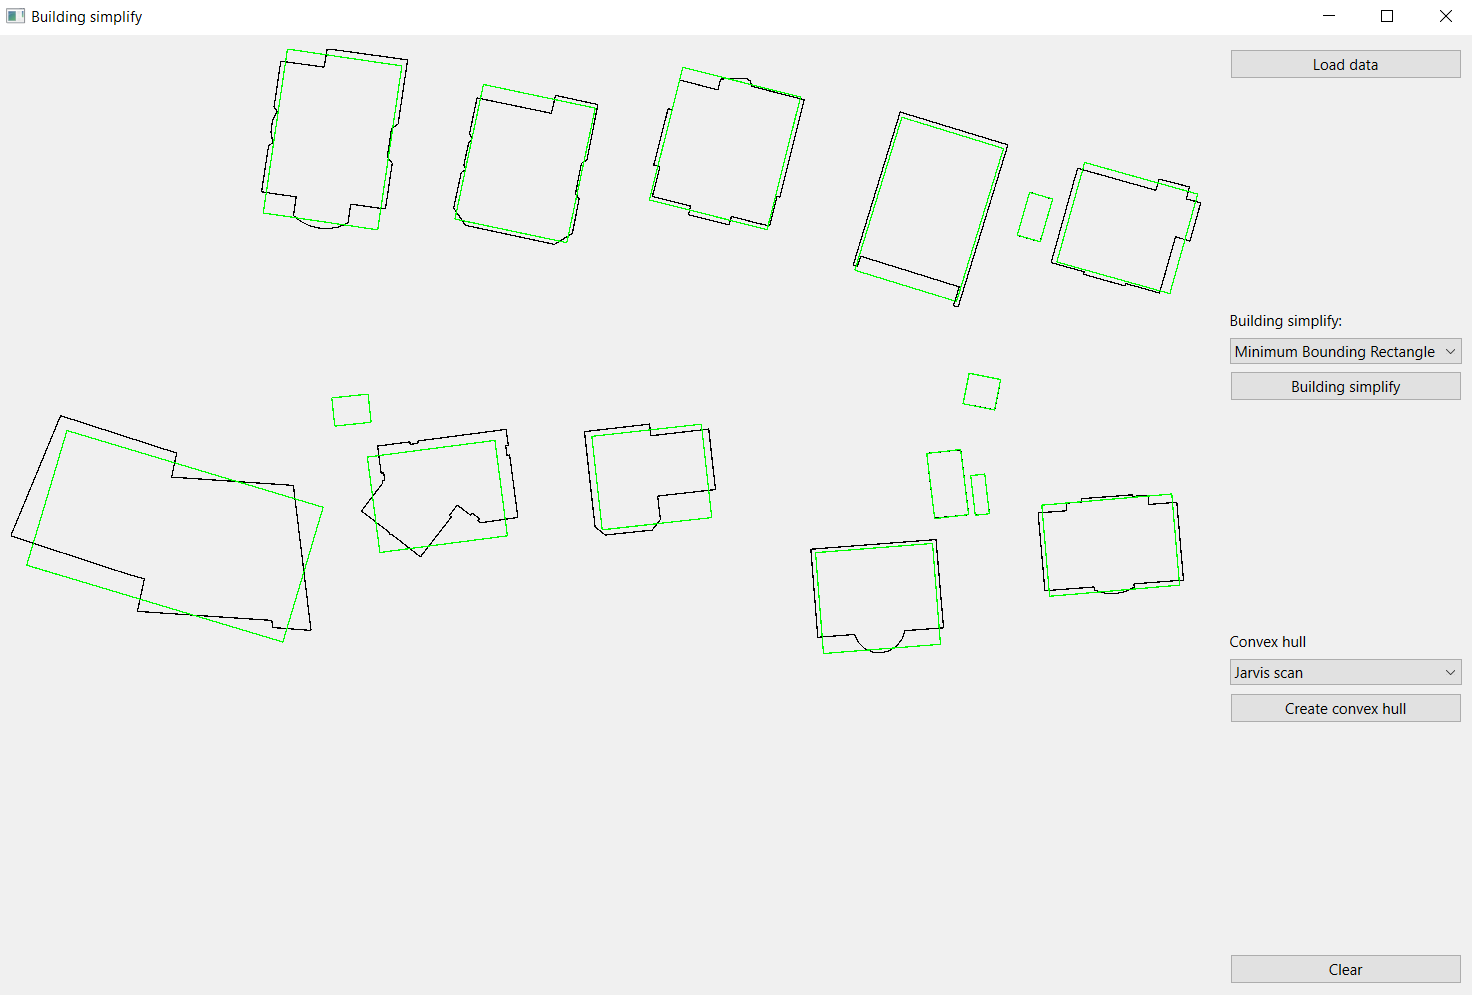
\includegraphics[scale=0.4]{images/U2_aplikace_MAER.png} 
			\caption{Minimum Area Enclosing Rectangle}
			\label{fig:app_MAER}
		\end{figure} 
		\begin{figure}[htbh]
			\centering
			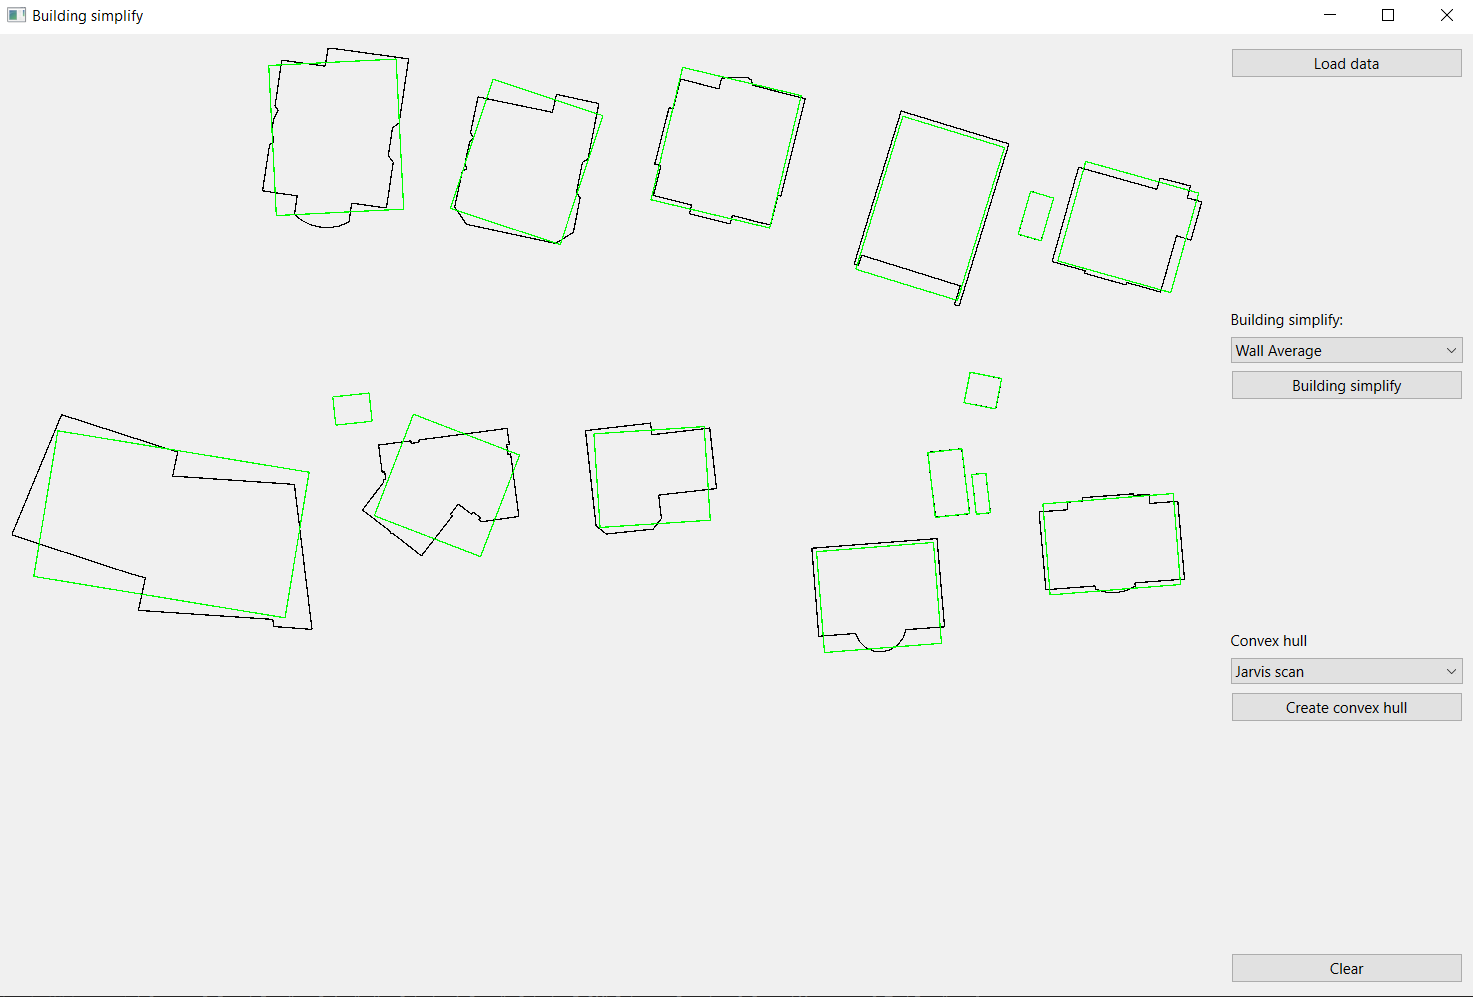
\includegraphics[scale=0.4]{images/U2_aplikace_WallAvarage.png} 
			\caption{Wall Avarage}
			\label{fig:app_WallAvarage}
		\end{figure} 
		\begin{figure}[htbh]
			\centering
			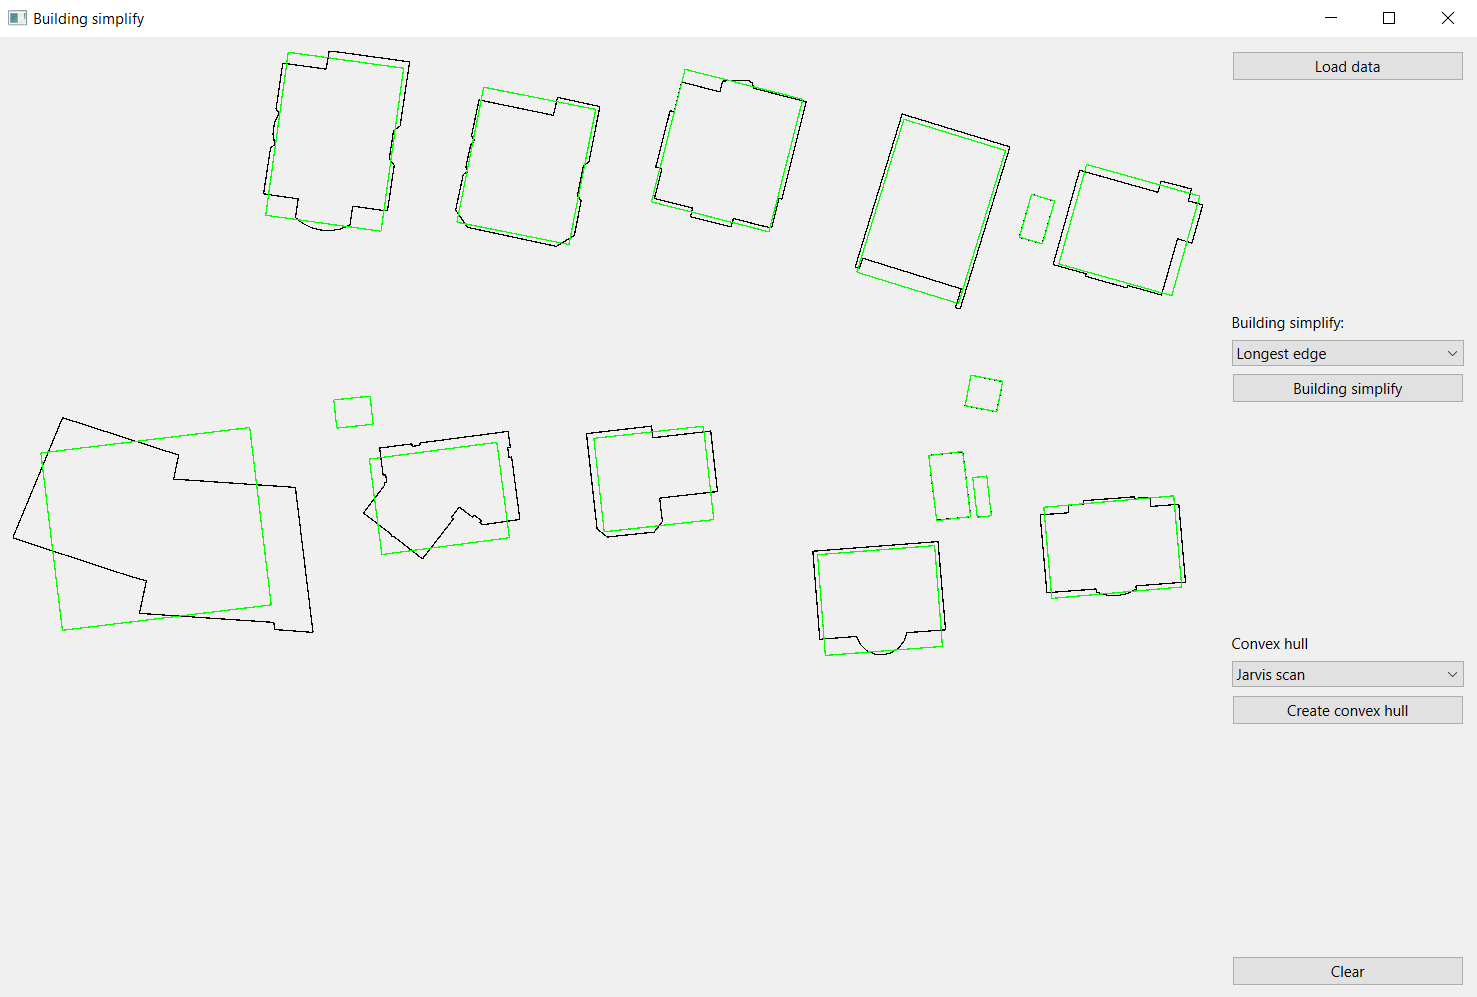
\includegraphics[scale=0.4]{images/U2_aplikace_LongestEdge.png} 
			\caption{Longest Edge}
			\label{fig:app_LongestEdge}
		\end{figure} \begin{figure}[htbh]
			\centering
			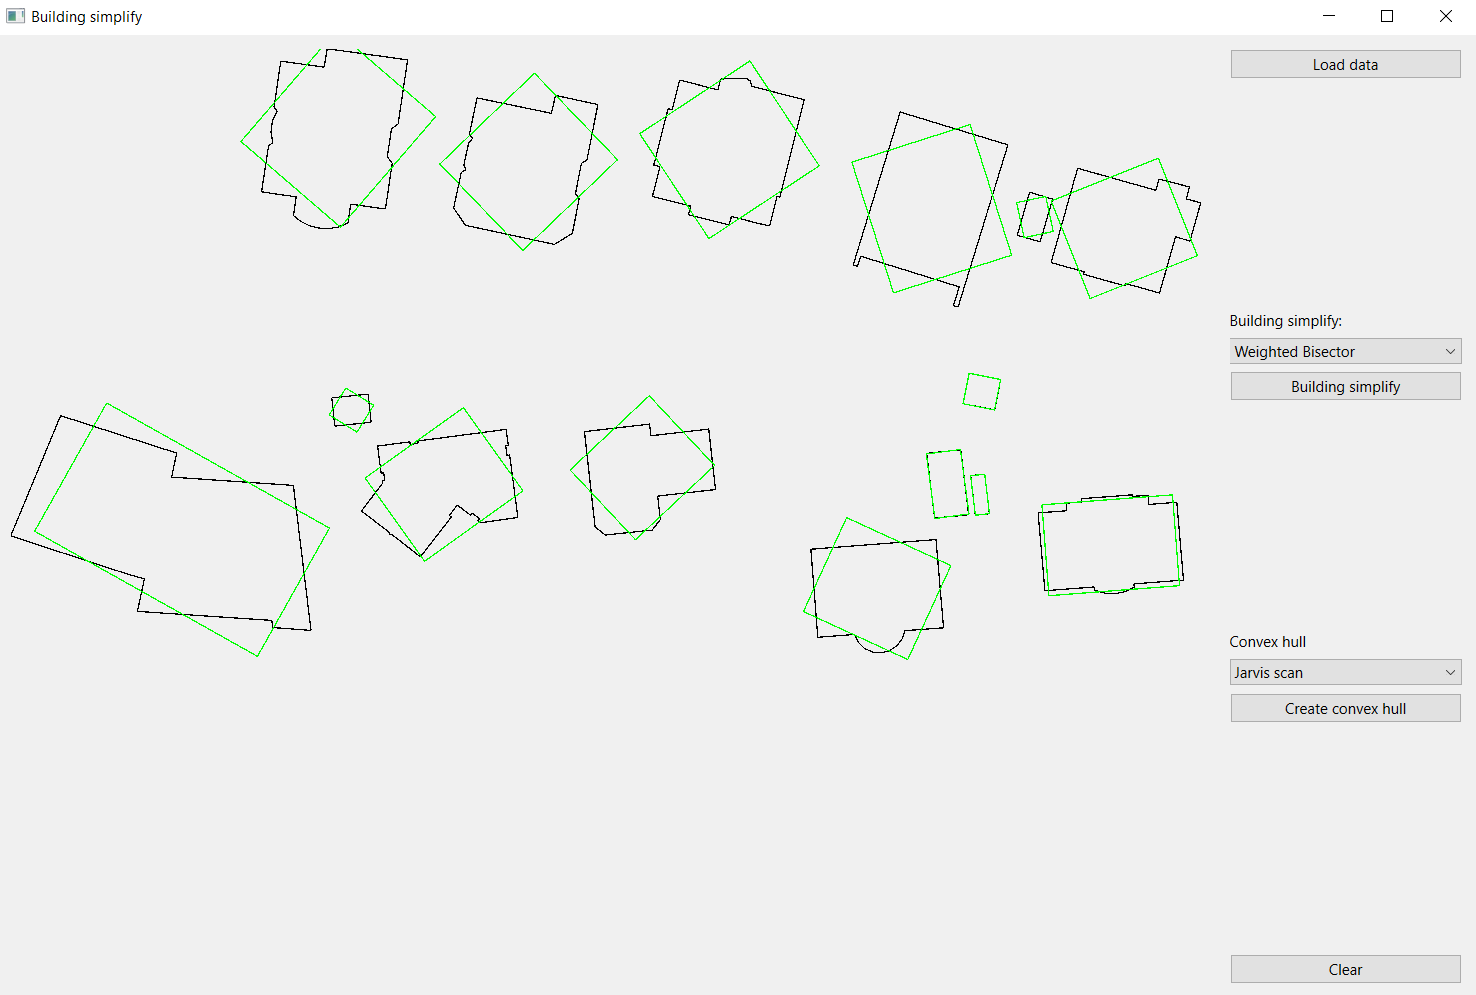
\includegraphics[scale=0.4]{images/U2_aplikace_WeightedBisector.png} 
			\caption{Weighted Bisector}
			\label{fig:app_WeightedBisector}
		\end{figure} 
		
		\clearpage
		
		\section{Printscreen vytvořené aplikace}
		\begin{figure}[htbh]
			\centering
			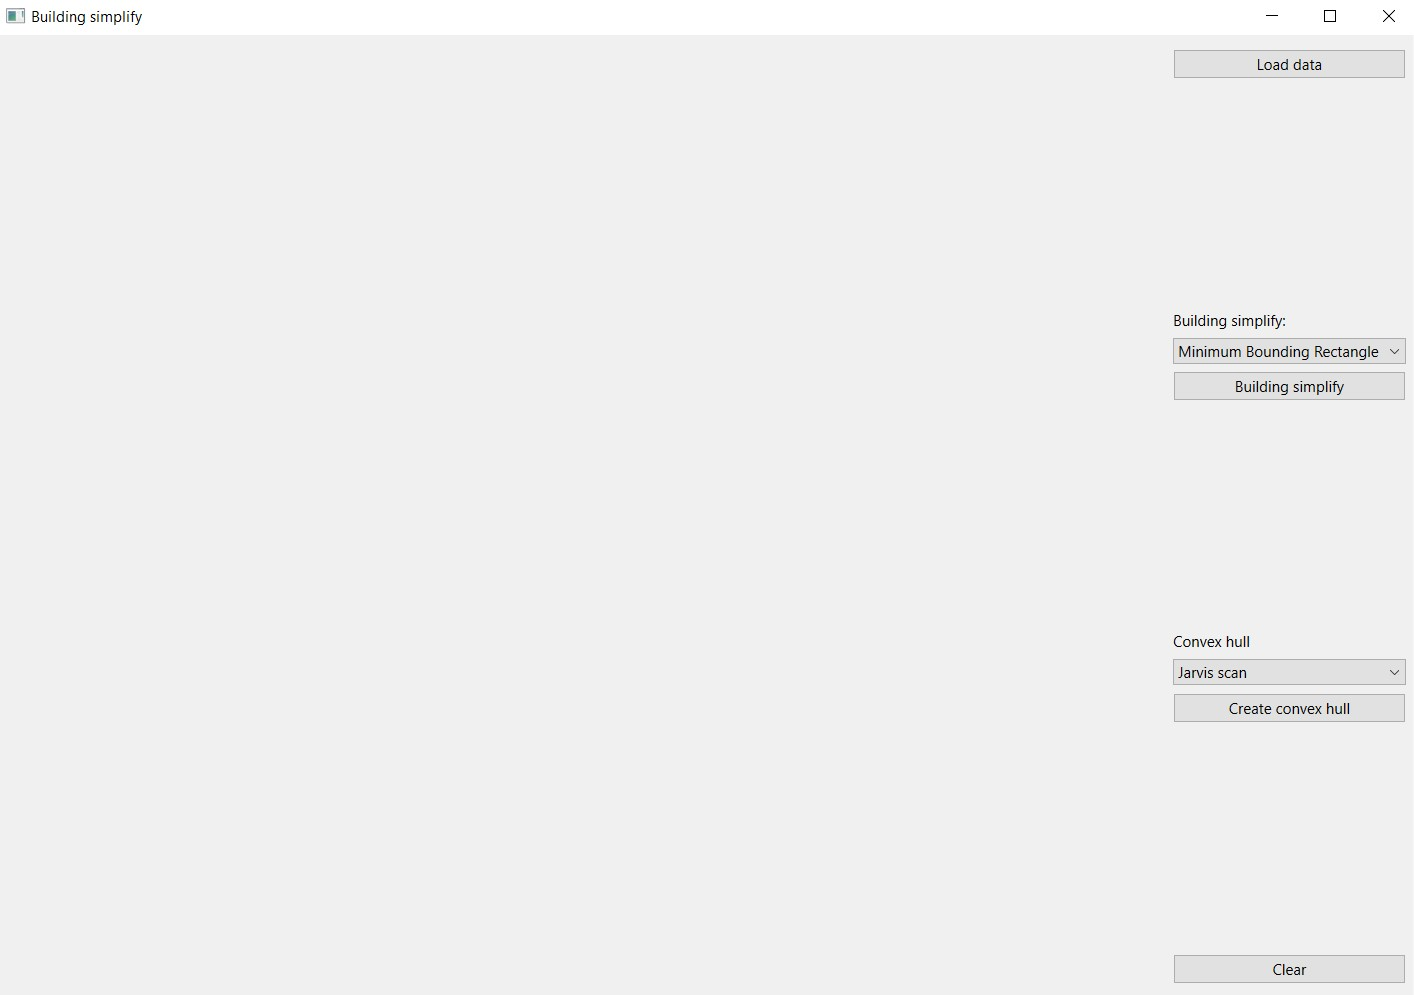
\includegraphics[scale=0.4]{images/U2_aplikace_uvodni_okno.jpg} 
			\caption{Úvodní okno aplikace}
			\label{fig:uvodni_okno}
		\end{figure} 
		
		%----------------------------------------------------------------------------------------
		%	DOKUMENTACE
		%----------------------------------------------------------------------------------------
		
		\section{Dokumentace}
		Kód zahrnuje 5 tříd – Algorithms, Draw, SortByX, SortByY a Widget, které budou následně detailněji popsány.      
		
		\subsection{Třída Algorithms}
		Třída Algorithms obsahuje 4 funkce :  
		
		\begin{itemize}
			\item double get2LinesAngle(QPoint \&p1, QPoint \&p2, QPoint \&p3, QPoint \&p4);
			\item int getPointLinePosition(QPoint \&a, QPoint \&p1, QPoint \&p2);
			\item double getPointLineDistance(QPointF \&a, QPointF \&p1, QPointF \&p2);
			\item QPolygonF cHull (std::vector <QPointF> \&points);
			\item QPolygonF qHull (std::vector <QPointF> \&points);
			\item void qHullRecursive(int r, int s, std::vector<QPointF> \&points, QPolygonF \&ch);
			\item std::vector <QPointF> rotate(std::vector <QPointF> \&points, double sigma);
			\item std::tuple<std::vector<QPointF>, double> minMaxBox(std::vector <QPointF> \&points);
			\item QPolygonF minAreaEnclosingRectangle(std::vector <QPointF> \&points);
			\item QPolygonF wallAverage(std::vector <QPointF> \&points);
			\item QPolygonF longestEdge(std::vector <QPointF> \&points);
			\item QPolygonF weightedBisector(std::vector <QPointF> \&points);
			\item double LH(std::vector <QPointF> \&points);
			\item std::vector <QPointF> resizeRectangle(std::vector <QPointF> \&points, std::vector <QPointF> \&er);
		\end{itemize}
		
		\paragraph{double get2LinesAngle(QPoint \&p1, QPoint \&p2, QPoint \&p3, QPoint \&p4);}
		Počítá úhel mezi dvěma liniemi pomocí vztahu \ref{WN:omega_i}. Vstupními argumenty jsou body určující linie, tzn. vrcholy polygonu. Návratovou hodnotou funkce je double – desetinné číslo s velikostí úhlu mezi těmito přímkami.  
		
		\paragraph{int getPointLinePosition(QPoint \&a, QPoint \&p1, QPoint \&p2);}
		Analyzuje vzájemnou polohu mezi bodem a linií polygonu, resp. v jaké polorovině vůči linii se bod nachází. Vstupními argumenty funkce jsou souřadnice určovaného bodu (jako QPoint) a souřadnice 2 bodů určujících polohu linie (vrcholy polygonu taktéž jako QPoint). Funkce vrací vždy hodnotu 1, 0 nebo -1 dle následujících pravidel:
		
		\begin{itemize}
			\item 0 v případě, že bod leží v pravé polorovině,
			\item 1 v případě, že  bod leží v levé polorovině,
			\item -1 v případě, že bod leží na linii.
		\end{itemize}
		
		\paragraph{double getPointLineDistance(QPointF \&a, QPointF \&p1, QPointF \&p2);}
		Počítá vzdálenost mezi bodem a přímkou definovanou dvěma vrcholy polygonu. Vstupní hodnoty jsou 3 body datového typu QpointF. 
		
		\subsection{Třída Algorithms}
		\paragraph{QPolygonF cHull (std::vector <QPointF> \&points)}\mbox{}\\
		Funkce vytváří konvexní obálku metodou Jarvis scan popsanou v kapitole 4.1.1. Vstupním argumentem funkce je vektor obsahující body množiny \textit{S}, body jsou uloženy jako \textit{QPointF}. 	Návratovým typem funkce je \textit{QPolygonF}, tedy polygon se souřadnicemi uloženými s přesností float obsahující souřadnice vrcholů vypočtené konvexní obálky.
		
		\paragraph{QPolygonF qHull (std::vector <QPointF> \&points)}\mbox{}\\
		Funkce vytváří konvexní obálku metodou Quick Hull popsanou v kapitole 4.1.2. Vstupním argumentem funkce je vektor obsahující body množiny \textit{S}, které jsou uloženy jako \textit{QPointF}. Návratovým typem funkce je \textit{QPolygonF}, tedy polygon se souřadnicemi uloženými s přesností float, který obsahuje souřadnice vrcholů vypočtené konvexní obálky. 

		\paragraph{void qHullRecursive(int r, int s, std::vector<QPointF> \&points, QPolygonF \&ch)}\mbox{}\\
		Funkce je rekurzivní funkcí k výše uvedené funkci qHull. Touto funkcí se přidávají části konvexní obálky $\mathcal{H_U}$ a $\mathcal{H_L}$ do výsledné konvexní obálky $\mathcal{H}$.
	 	Vstupními argumenty jsou integery r a s, jež označují směr linie mezi pivoty \textit{$ q_1 $} a \textit{$ q_3 $}. Tyto body jsou uloženy ve vektoru \textit{points} (popsán níže) na prvních dvou místech, volá-li se tedy funkce například s těmito parametry: qHullRecursive(1,0,su,qh), bude počátečním bodem linie pivot \textit{$ q_3 $} a konečným bodem pivot \textit{$ q_1 $}. Třetím vstupním argumentem je vektor bodů \textit{QPointF} \textit{points}, do této proměnné se ukládá  $\mathcal{H_U}$ nebo $\mathcal{H_L}$. Posledním vstupním argumentem je \textit{QPolygonF}, do nějž se bude ukládat horní/spodní část konvexní obálky. Návratový typ funkce je void, funkce tedy nevrací žádnou proměnnou, pouze ukládá body do předem vytvořené proměnné.
	 	
	 	\paragraph{std::vector <QPointF> rotate(std::vector <QPointF> \&points, double sigma);}
	 	Otáčí množinu bodů u úhel sigma. Vstupními hodnotami jsou vektor bodů datového typu QPointF a úhel sigma, která vstupuje do transformační rovnice. Funkce opět vrací vektor bodů datového typu QPointF.
	 	
	 	\paragraph{std::tuple<std::vector<QPointF>, double> minMaxBox(std::vector <QPointF> \&points);}
	 	Vytváří kolem polygonu minimální ohraničující obdélník s vrcholy s extrémními souřadnicemi polygonu, nad kterým se obdélník vytváří. Vstupní hodnotou je vektor datového typu QPointF. Funkce vrací minimální ohraničující obdélník ve vektoru QPointF a jeho plochu s datovým typem double. Aby funkce mohla vracet dva objekty, je nutné je vracet jako tuple.
	 	
	 	\paragraph{QPolygonF minAreaEnclosingRectangle(std::vector <QPointF> \&points);}
	 	Generalizuje polygon, jehož hlavní směr je určen metodou Minimum Area Enclosing Rectangle. Hlavní směr je zde určen stranou konvexní obálky, která minimalizuje plochu minimální  ohraničujícího obdélníku otočeného o její směrnici. Do funkce vstupuje vektor datového typu QPointF a algoritmus vrací natočený obdélník, který je uložen v datovém typu QPolygonF.
	 	
	 	\paragraph{QPolygonF wallAverage(std::vector <QPointF> \&points);}
	 	Generalizuje polygon, jehož hlavní směr je určen metodou Wall Avarage, kde je hlavní směr dán váženým průměrem, do kterého vstupují směrnice první strany polygonu, rezidua po dělení směrnic hodnotou $\pi/2$ a délka strany. Do funkce vstupuje vektor datového typu QPointF a algoritmus vrací natočený obdélník, který je uložen v datovém typu QPolygonF.
	 	
	 	\paragraph{QPolygonF longestEdge(std::vector <QPointF> \&points);}
	 	Generalizuje polygon, jehož hlavní směr je určen metodou Longest Edge. Hlavní směr je zde představován nejdelší stranou budovy. Do funkce vstupuje vektor datového typu QPointF a algoritmus vrací natočený obdélník, který je uložen v datovém typu QPolygonF.
	 	
	 	\paragraph{QPolygonF weightedBisector(std::vector <QPointF> \&points);}
	 	Generalizuje polygon, jehož hlavní směr je určen metodou Weighted Bisector, která hlavní směr určuje váženým průměrem směrů dvou nejdelších úhlopříček. Do funkce vstupuje vektor datového typu QPointF a algoritmus vrací natočený obdélník, který je uložen v datovém typu QPolygonF.
	 	
	 	\paragraph{double LH(std::vector <QPointF> \&points);}
	 	Počítá plochu budovy pomocí L'Hullierova vzorce. Vstupní hodnotou je vektor datového typu QPointF, výstupní hodnotou je plocha budovy typu double.
	 	
	 	\paragraph{std::vector <QPointF> resizeRectangle(std::vector <QPointF> \&points, std::vector <QPointF> \&er);}
	 	Mění velikost generalizované budovy tak, aby se její plocha shodovala s plochou původní budovy. Vstupními hodnotami jsou vektor bodů datového typu QPointF představující původní budovu a vektor bodů datového typu QPointF představující generalizovanou budovu. Funkce vrací opět vektor bodů datového typu QPointF, který představuje generalizovanou budovu s plochou odpovídající původní budově.s
	 	
	 	
	 	\subsection{Třída Draw}
	 	Třída Draw obsahuje následující funkce, které budou dále podrobně popsány:
	 	
	 	\begin{itemize}
	 		\item void paintEvent(QPaintEvent *event);
	 		\item void clear();
	 		\item QPoint getPoint(){return q;}
	 		\item std::vector<QPolygonF> getPolygons()\{return buildings;\}
	 		\item void setCh(std::vector <QPolygonF> \&ch\_\{chs = ch\_;\}
	 		\item void setEr(std::vector <QPolygonF> \&er\_)\{ers = er\_;\}
	 		\item void loadData(QString \&file\_name);
	 	\end{itemize}
	 	
	 	a následující proměnné:
	 	
	 	\begin{itemize}
	 		\item std::vector<QPointF> points;
	 		\item std::vector <QPolygonF> ers, chs;
	 		\item std::vector <QPolygonF> buildings;
	 		\item QPointF p;
	 		\item double y\_max = 0, x\_min = 999999999;
	 		\item double y\_min = 999999999, x\_max = 0;
	 	\end{itemize}
	 	
	 	\paragraph{•	void paintEvent(QPaintEvent *event);}\mbox{}\\
	 	Funkce nastavuje grafické atributy vykreslovaných objektů a kreslí na plátno zadané polygony, jejich konvexní obálku a jejich generalizaci. 
	 	
	 	\paragraph{void clear();}\mbox{}\\
	 	Funkce smaže veškeré objekty, jež jsou vykresleny na plátně. Funkce nemá vstupní argumenty. 
	 	
	 	\paragraph{std::vector<QPolygonF> getPolygons()\{return buildings;\}}
	 	
	 	Funkce vrací vektor polygonů načtených z textového souboru – návratový typ je std::vector<QPolygon>, funkce nemá vstupní argumenty.
	 	
	 	\paragraph{void setCh(std::vector <QPolygonF> \&ch\_\{chs = ch\_;\}}
	 	
	 	\paragraph{void setEr(std::vector <QPolygonF> \&er\_)\{ers = er\_;\}}
	 	
	 	\paragraph{void loadData(QString \&file\_name);}\mbox{}\\
	 	Funkce načítá data z textového souboru a ukládá je do vektoru QPolygonF. Funkce také rovnou transformuje souřadnice s S-JTSK do souřadnicového systému plátna. Vstupní argumentem je cesta k souboru, jejž chceme načíst do aplikace.   
	 	
	 	\subsection{Třída SortByX}
	 	Řadí body podle xové souřadnice.
	 	
	 	\subsection{Třída SortByY}
	 	Řadí body podle y-ové souřadnice.
	 	
	 	\subsection{Třída Widget}
	 	Třída Widget obsahuje 3 metody:
	 	
	 	\begin{itemize}
	 		\item void on\_pushButtonClear\_clicked();
	 		\item void on\_pushButtonSimplify\_clicked();
	 		\item void on\_pushButtonLoadData\_clicked();
	 		\item void on\_pushButtonConvexHull\_clicked();
	 		
	 	\end{itemize}
	 	
	 	\paragraph{ void on\_pushButtonClear\_clicked();}\mbox{}\\
	 	Funkce se volá při stisknutí tlačítka Clear, volá funkci clear(), jež je definovaná v třídě Draw.
	 	
	 	\paragraph{ void on\_pushButtonAnalyze\_clicked();}\mbox{}\\
	 	Funkce se volá při stisknutí tlačítka Building simplify a provádí jednotlivé metody generalizace budov na základně indexu v comboboxu. 
	 	
	 	\paragraph{void on\_pushButtonLoad\_clicked();}\mbox{}\\
	 	Funkce slouží k inicializaci načítání souboru, spustí se po stisknutí tlačítka Load, čímž zobrazí dialog pro výběr souboru obsahujícího data, jež mají být načtena do aplikace. Po výběru souboru se zavolá funkce loadData ze třídy Draw, která přečte data ze souboru a uloží je do proměnné.
	 	
		
		%----------------------------------------------------------------------------------------
		%	ZÁVĚR
		%----------------------------------------------------------------------------------------
		
		\section{Závěr}
		
		
		

		
	\end{document}